\documentclass{beamerhpi}

% title: [content slides]{title slide}
\title[Quantum Programming - qPCA]{Quantum Programming - Implementing a quantum based Principal Component Analysis}
% date: {content slides}
\date{03. September 2021}
% author: [content slides]{title slide}
\author[Raschack Selina]{Speaker\texorpdfstring{\\}{, }Job Description}
% institute: {title slide}
\institute{Quantum Programming WiSe 2020/21}
\usepackage{lmodern}
\boolfalse{fakultaet} % use \booltrue instead of \boolfalse if you are creating an official faculty presentation
% for crazy demands like captions for images in minipages
\usepackage{caption}
% Uncomment the following three lines to generate notes from \note command on the right side, which can be displayed with pympress ( https://github.com/Cimbali/pympress )
% \usepackage{pgfpages}
% \setbeamertemplate{note page}[plain]
% \setbeameroption{show notes on second screen=right}


\usepackage{url}
\usepackage{amsmath}


\begin{document}

	\begin{frame}[title={bg=Hauptgebaeude_Nacht}]
		\maketitle
	\end{frame}

	\begin{frame}{Agenda}
  \begin{minipage}{1.0\textwidth}
    \begin{itemize}
      \item Context
      \begin{itemize}
        \item notations
        \item classical PCA
        \item quantum PCA
      \end{itemize}
      \item Implementation
          \begin{itemize}
            \item circuit initialization
            \item simple quantum PCA with swap test
            \item enhancements with quantum phase estimation
          \end{itemize}
      \item Results
      \item Conclusion
    \end{itemize}
  \end{minipage}
\end{frame}

	1. Quantum Computing

[yanofsky paper - begin]
\begin{description}
  \item[Quantum system] A quantum system is a system with its state and transitions not being deterministic. Furthermore, the probabilities of states and transitions are given as complex numbers $c$ such that $|c|^2$ is a real number between $0$ and $1$.
  \item[Qubits] In quantum computing the concept of bits is extended to the so called \emph{quantum bits} or \emph{qubits}. A \emph{qubit} can be any state that can be represented as:
    \[
      \begin{matrix} 0 \\ 1 \end{matrix}
      \begin{bmatrix} c_0 \\ c_1 \end{bmatrix}
      \text{, where }
      |c_0|^2 + |c_1|^2 = 1 \text{ and } c_0, c_1 \in \mathbb{C}
    \]
\end{description}
Note that from the previous introduced definition of a \emph{quantum system} the probabilities of states and transitions are complex numbers that should comply to the constrain that their square product leads to real number between $0$ and $1$. To perform these state transitions quantum operations are defined from quantum gates:
\begin{description}
\item[Quantum Gates] A quantum gate is any unitary matrix that manipulates qubits. [double check if unitary is the only required attribute]
\end{description}

-- Hadamard gate and R_y gate as examples -> will be referenced for the types of measurements
[yanofsky paper - end]

[qiskit textbook - begin]
A common notation is the so called \emph{bra ket} notation: [example]. To chain different gates to build more complex oprations the \emph{outer product} or \emph{matrix multiplication) is applied: [example].

To represent a quantum state the \emph{quantum state vector} or a \emph{density matrix} can be used. The \emph{ket} notation refers to a column state vector and the \emph{bra} notation to a transposed column state vector (row vector). Therefore, the density matrix can be noted as [ket bra notation here].

--- diff types of measurements (diff bases)
[qiskit textbook - end]

Complete randomness or increasment in computation speed are two goals commonly assigned with quantum computing. To achieve these goals the following concepts from quantum mechanics are applied:

[mooc begin]
\begin{description}
  \item[Superposition] With the given representation of a qubit it is possible to create a quantum state that is a combination of $|0\rangle$ and $|1\rangle$:
    \[
      \begin{bmatrix} c_1 \\ c_2 \end{bmatrix} = c_1 |0\rangle + c_2 |1\rangle
    \]
    If $c_1$ and $c_2$ are non-zero, the qubit's state contains both $|0\rangle$ and $|1\rangle$ at the same time which is called superposition. --> reference hadamard gate here.

  \item[Entanglement] With two qubits a quantum state can be represented as a combination of:
    \[
      c_1|00\rangle + c_2|01\rangle + c_3|10\rangle + c_4|11\rangle
    \]
    where $|c_1|^2 + |c_2|^2 + |c_3|^2 + |c_4|^2 = 1$, $c_1, c_2, c_3, c_4 \in \mathbb{C}$ and where $|01\rangle$ means the first qubit is in state $|0\rangle$ and the second qubit is in state $|1\rangle$. If two or more of the complex factors are non-zero it is not possible to separate the qubits.
[mooc - end]


2. Engineering
- goal
- how to approach

2.2 Circuit initialization techiques
-- bitwise
-- amplitude stuff
-- purifying / reduced density matrix


3. PCA
In this paper the \epmh{Principal Component Analysis} (PCA) will be used as a target problem to solve. The algorithm can be used on high-dimensional data to extract the $n$ most significant features and reduce the total number of dimensions and therefore the complexity of a given data set.

In their paper \enquote{A Tutorial on Principal Component Analysis} (\cite{Shlens, 2014}) Shlens gives an in-depth but applied approach into PCA. The discussed concepts and steps in classical PCA do reflect to the different quantum based PCA solutions proposed by the research community.

- Redundancy > Covariance Matrix > Diagonalize the covariance Matrix
=> classical preprocessing, classical prerpocessing, swap test [?]

- eigenvector decomposition
=> 

- singular value decomposition
=> 



Ref
- yanofsky paper
- qiskit textbook -> ref the relevant articles
- mooc
Shlens (2014): A Tutorial on Principal Component Analysis (arXiv: 14041100v1)

	\begin{frame}[title-small={color=hpiorange, bg=none, text=Implementation}]
	\maketitle
\end{frame}


\begin{frame}{Circuit Initialization - Classical Register (Bit-wise)}
  \begin{minipage}{1.0\textwidth}
    \begin{itemize}
      \item idea: describe classical state as bit string of length n and use register of $n$ qubits to represent as quantum state
      \item easy to implement, easy to measure
      \item limitations: large amount of qubits needed $\rightarrow$ hardware limitations, circuit complexity
      \item related works: [Corte2018] $\rightarrow$ reduce number of qubits, discard operations
    \end{itemize}
  \end{minipage}
\end{frame}


\begin{frame}{Circuit Initialization - State Purification \& Schmidt decomposition}
  \begin{minipage}{1.0\textwidth}
    \begin{itemize}
      \item idea: describe a classical state as pure or mixed quantum state via density operation $\rho$
      \begin{itemize}
        \item pure state: $\rho = \Sigma_{i=1}^{n} |\psi\rangle \langle\psi |$, trace $Tr(\rho) = 1$
        \item mixed state: $\rho = \Sigma_{i=1}^{n} p_i |\psi_i\rangle \langle\psi_i |$, trace $Tr(\rho) < 1$
      \end{itemize}
      \item reduced density operation: two systems $A$ and $B$, then $\rho_{A} = Tr_B(\rho_{AB})$
      \begin{itemize}
        \item describe entangled states
        \item state purification: system $A$ in a mixed state $\rightarrow$ a composed system $AB$ can be found that complies with the reduced density operation $\rho_{A}$ and $AB$ in a pure state
      \end{itemize}
			\item state preparation: use Schmidt decomposition to compute the unitary preparion operation:
			\begin{itemize}
				\item $U_{prep} = (U_A \otimes U_B) CNOT_{AB} (U_{A}^{'} \otimes I_B )$
			\end{itemize}
    \end{itemize}
  \end{minipage}
	\begin{minipage}{1.0\textwidth}
    \centering
    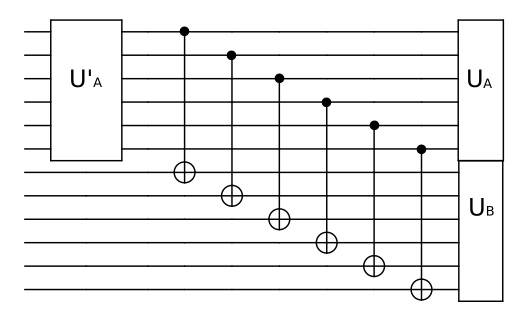
\includegraphics[width=0.3\textwidth]{../assets/schmidt_decomposition_main-ref19.png}
  \end{minipage}
	\footnote{[Lokho2020], [Niels2010]}
\end{frame}


\begin{frame}{Circuit Initialization - Amplitude Amplification}
  \begin{minipage}{0.5\textwidth}
    \begin{itemize}
      \item idea: "search" the quantum state via grover algorithm
      \begin{itemize}
        \item step 1: start in the uniform superposition $|s\rangle = H^{\otimes n}$
        \item step 2: apply oracle operation $U_f$
        \item step 3: apply reflection operation $U_s$, $U_s=2|s\rangle \langle s| -1$
      \end{itemize}
    \end{itemize}
  \end{minipage}%
  \hfill
  \begin{minipage}{0.5\textwidth}
    \centering
    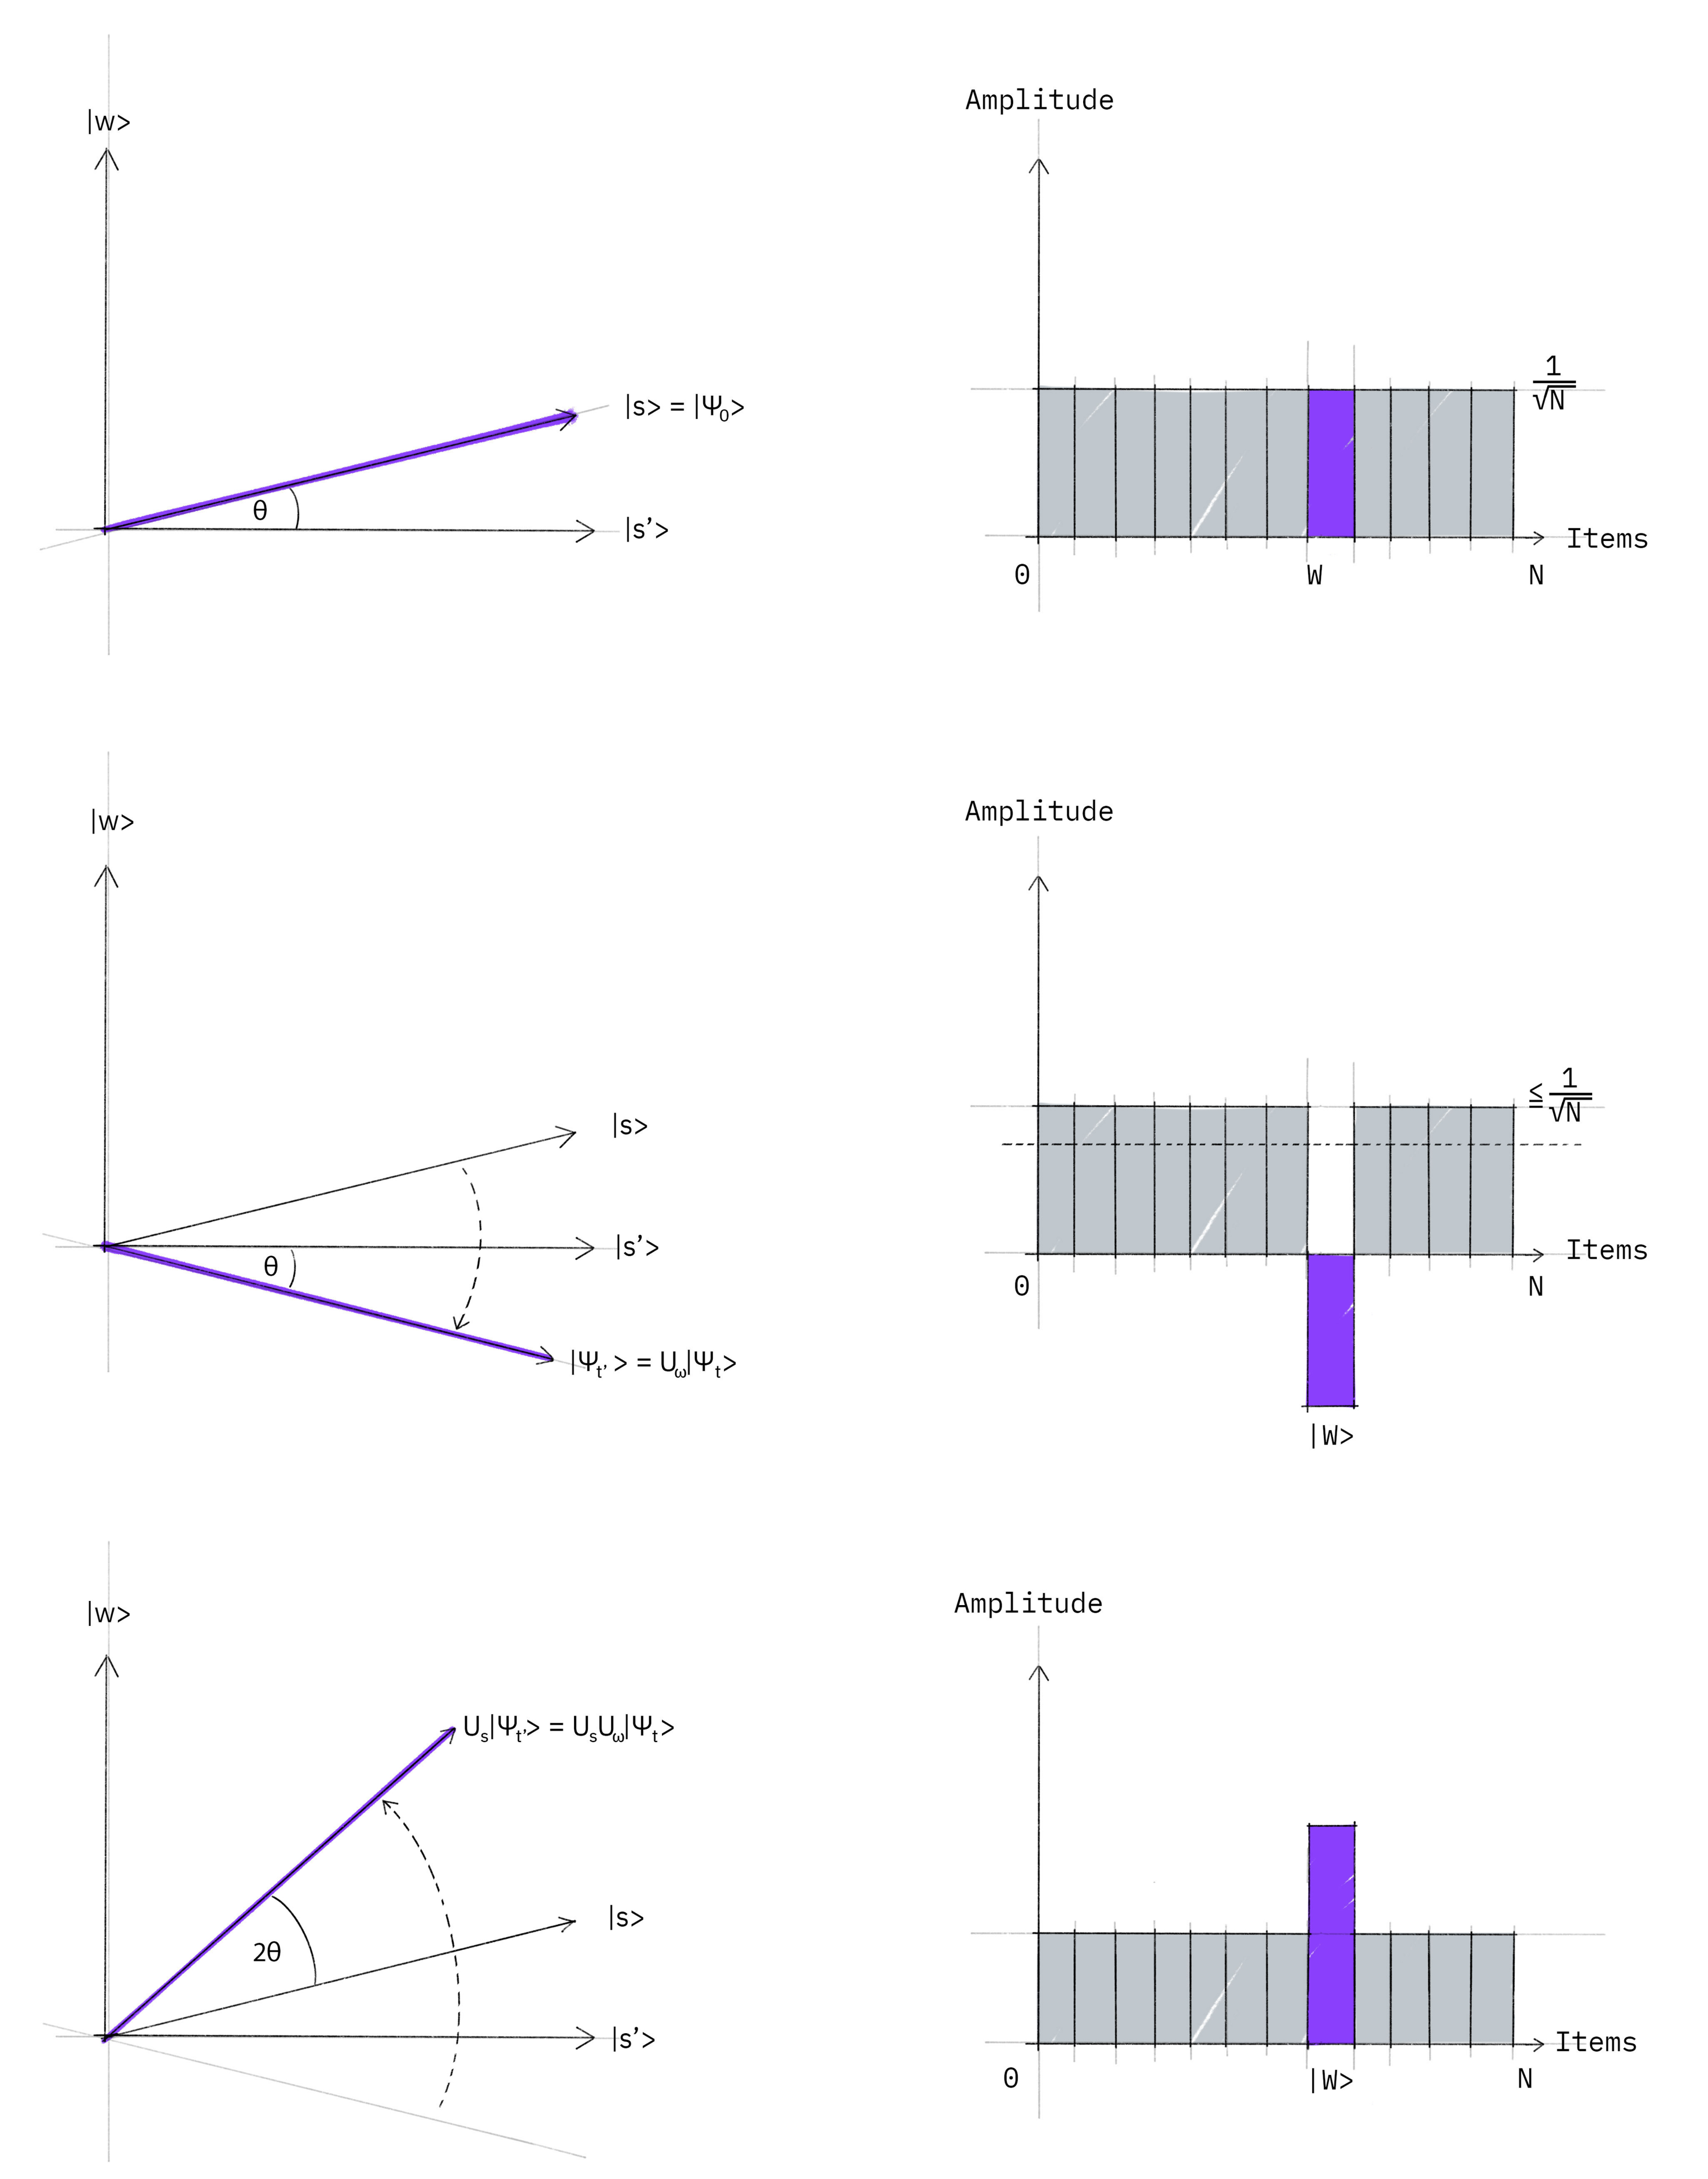
\includegraphics[width=0.8\textwidth]{../assets/grover_steps.png}
  \end{minipage}
  \footnote{[Daski2015], \url{https://qiskit.org/textbook/ch-algorithms/grover.html}}
\end{frame}


\begin{frame}{Circuit Initialization ~ Challenges}
  \begin{minipage}{1.0\textwidth}
    \begin{itemize}
      \item textbook examples often quantum states that are easy to implement, e.~g. classical states
      \item paper examples often very brief description how to initialize quantum state
      \item method specifics:
      \begin{itemize}
        \item bit-wise: properly apply discard operations
        \item state purification: find composed state in respect to the density matrix of given data set
        \item amplitude amplification: find oracle operation in respect to the given data set
      \end{itemize}
    \end{itemize}
  \end{minipage}
\end{frame}


\begin{frame}{Simple Quantum PCA with Swap Test}
  \begin{minipage}{1.0\textwidth}
    \begin{itemize}
      \item used libraries: python, unittest, numpy, cirq
      \item cirq testing: package cirq.testing
      \begin{itemize}
        \item assert\_same\_circuits $\rightarrow$ tests if two circuits are \emph{equivalent} to each other
        \item assert\_has\_diagram $\rightarrow$ tests the text representation
      \end{itemize}
    \end{itemize}
  \end{minipage}
  \begin{minipage}{1.0\textwidth}
    \centering
    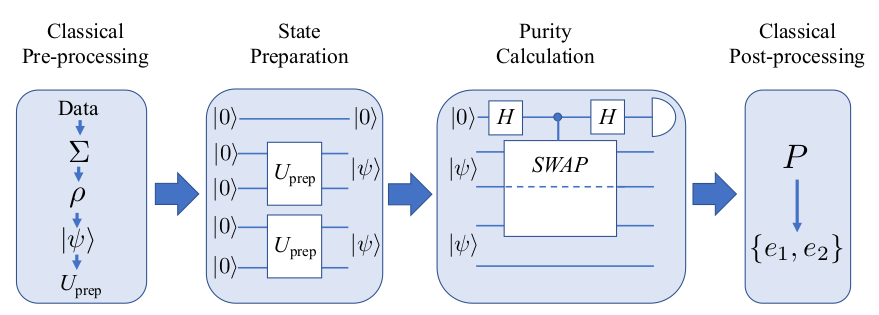
\includegraphics[width=0.8\textwidth]{../assets/context_algorithm_main-ref19.png}
  \end{minipage}
\end{frame}


\begin{frame}{Simple Quantum PCA with Swap Test - State Preparation}
  \begin{minipage}{0.5\textwidth}
    \begin{itemize}
      \item cirq: gate vs. operation vs. circuit
      \begin{itemize}
        \item implementation circuit initialization: internal method of "SimpleSwapTestQPCA" cirq circuit
        \item unitary preparation operation to initialize $|\psi\rangle$ can be computed independently
        \item circuit makes sure enough copies of $|\psi\rangle$ are initialized
      \end{itemize}
    \end{itemize}
  \end{minipage}%
	\begin{minipage}{0.5\textwidth}
    \centering
    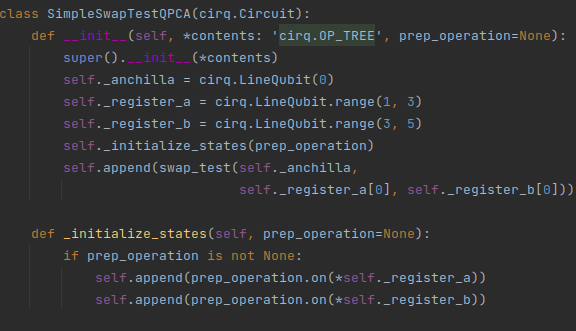
\includegraphics[width=1.0\textwidth]{../assets/code-snippet_simple_circuit.png}
  \end{minipage}
\end{frame}


\begin{frame}{Simple Quantum PCA with Swap Test - Purify Calculation}
  \begin{minipage}{0.5\textwidth}
    \begin{itemize}
      \item swap test: operation to check level of difference of two quantum states
      \begin{itemize}
        \item input: two quantum states, each represented with $n$ qubits
        \item output: level of equality of the two states
      \end{itemize}
      \begin{itemize}
        \item if both states are orthogonal to each other: probability to measure $0$ is $\frac{1}{2}$
        \item if both states are equal to each other: probability to measure $0$ is $1$
      \end{itemize}
    \end{itemize}
  \end{minipage}%
  \begin{minipage}{0.5\textwidth}
    \centering
    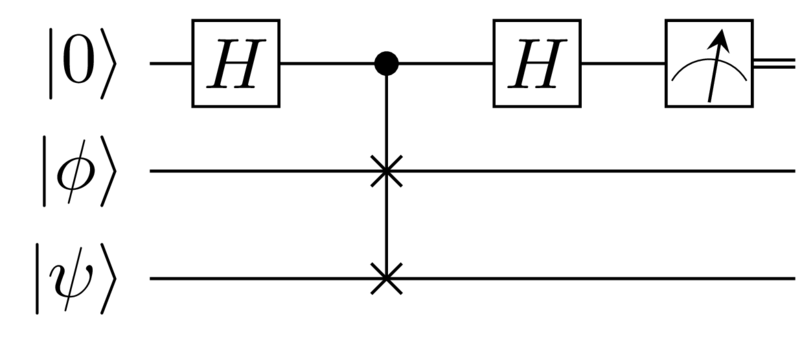
\includegraphics[width=0.8\textwidth]{../assets/wp_swap_test_simple.png}
  \end{minipage}
  \footnote{\url{https://en.wikipedia.org/wiki/Swap_test}}
\end{frame}


\begin{frame}{Simple Quantum PCA with Swap Test - Purify Calculation}
  \begin{minipage}{0.5\textwidth}
    \begin{itemize}
      \item cirq: gate vs. operation vs. circuit
      \begin{itemize}
        \item implementation swap test: cirq gate "SwapTestGate" and "swap test" function which returns a cirq operation
        \item drawback: gates only know qubits but not register of qubits $\rightarrow$ swap test composition makes some assumptions how qubits are entered into the gate
        \item better: directly implement as cirq operation
      \end{itemize}
      \item cirq: equality vs. value equality
      \item end-to-end testing: simulate circuit $\rightarrow$ find acceptable delta between expected and actual result
    \end{itemize}
  \end{minipage}%
	\begin{minipage}{0.5\textwidth}
    \centering
    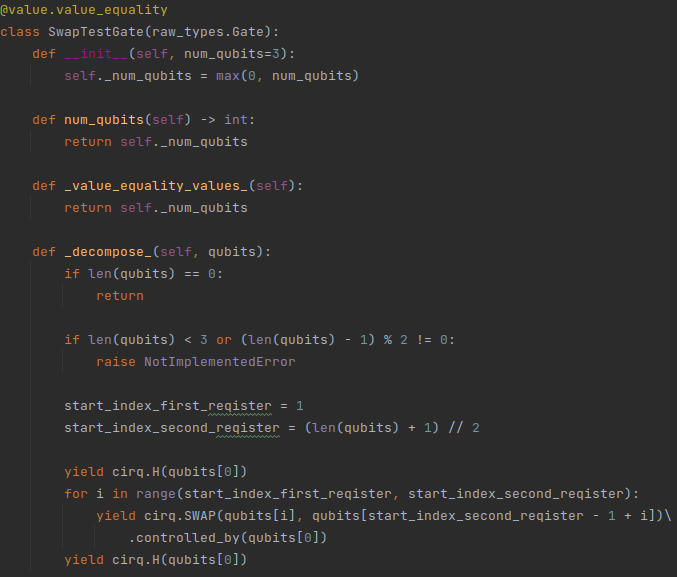
\includegraphics[width=1.0\textwidth]{../assets/code-snippet_swap-gate.png}
  \end{minipage}
\end{frame}


\begin{frame}{Simple Quantum PCA with Swap Test - Post-processing}
  \begin{minipage}{1.0\textwidth}
    \begin{itemize}
      \item formula to calculate the two eigenvalues\footnote{[Lokho2020]} with purity $P = Tr(\rho^2)$:
      \begin{itemize}
        \item $e_1 = Tr(\Sigma) \ast (1 + \sqrt{1 - 2 (1 - P)}) / 2$
        \item $e_2 = Tr(\Sigma) \ast (1 - \sqrt{1 - 2 (1 - P)}) / 2$
      \end{itemize}
      \item this formula is specific for $2 \times 2$ matrices and maybe even mixed states
      \item example from [He2021]: formula does not calculate eigenvalues correctly
    \end{itemize}
  \end{minipage}
\end{frame}


\begin{frame}{Enhancements with Quantum Phase Estimation}
  \begin{minipage}{1.0\textwidth}
    \centering
    
\includegraphics[width=0.7\textwidth]{../assets/wp_phase_estimation.png}
  \end{minipage}
  \footnote{\url{https://en.wikipedia.org/wiki/Quantum_phase_estimation_algorithm}}
  \begin{minipage}{1.0\textwidth}
    \begin{itemize}
      \item more generalized circuit for quantum based eigenvalue calculation
      \item algorithm can calculate $n$ eigenvalues not only two
      \item changes in the preprocessing: need to compute unitary operation for the QPE
      \item changes in the post-processing: calculate eigenvalues from amplitudes
    \end{itemize}
  \end{minipage}
\end{frame}

	\begin{frame}[title-small={color=hpiorange, bg=none, text=Results}]
	\maketitle
\end{frame}


\begin{frame}{Results}
  \begin{minipage}{1.0\textwidth}
    (switch to jupyter notebook)
  \end{minipage}
\end{frame}

	\begin{frame}[title-small={color=hpiorange, bg=none, text=Conclusion}]
	\maketitle
\end{frame}


\begin{frame}{Conclusion}
  \begin{minipage}{1.0\textwidth}
    \begin{itemize}
      \item different algorithms for qPCA have been proposed by research community $\rightarrow$ often additional constraints for practical implementing
      \begin{itemize}
        \item types of limitations discussed: number of qubits, qubit layout, circuit depth, circuit noise
      \end{itemize}
      \item integration: quantum state initialization is a non-trivial task when implementing and testing quantum algorithms
      \begin{itemize}
        \item three techniques discussed: classical register, density matrix, amplitude amplification
      \end{itemize}
      \item design: support through the different high-level libraries
      \begin{itemize}
        \item python cirq library discussed: circuit, operation, gate, value equality, testing
      \end{itemize}
    \end{itemize}
  \end{minipage}
\end{frame}


\begin{frame}{Conclusion}
  \begin{minipage}{1.0\textwidth}
    \begin{itemize}
      \item implementation: support through the different high-level libraries
      \begin{itemize}
        \item python unit-testing and end-to-end component testing discussed: classical assertions, circuit simulation
        \item not discussed: other types of testing for quantum algorithms, e.~g. projection based runtime assertions
        \item not discussed: error code correction to address noise or mixed states
      \end{itemize}
      \item maintenance: enhancements on the simple qPCA algorithm applied
      \begin{itemize}
        \item types of effects / changes discussed: preprocessing, post-processing, testing
      \end{itemize}
    \end{itemize}
  \end{minipage}
\end{frame}

	\begin{frame}{References}
  \begin{minipage}{1.0\textwidth}
    \begin{itemize}
      \item paper:
      \begin{description}
        \item [\text{[}Shlen2014\text{]}] J. Shlens (2014): "A Tutorial on Principal Component Analysis" (arXiv: 1404.1100v1)
        \item [\text{[}Melke2010\text{]}] D. v. Melkebeek (2010): \emph{CS 880: Quantum Information Processing}, "Lecture 20: Density Operator Formalism"
        \item [\text{[}He2021\text{]}] He et.~al. (2021): "A Low Complexity Quantum Principal Component Analysis Algorithm" (arXiv: 2010.00831v2)
        \item [\text{[}Lokho2020\text{]}] Lokhov et.~al. (2020): "Quantum Algorithm Implementations for Beginners" (arXiv: 1804.03719v2)
        \item [\text{[}Corte2018\text{]}] J. A. Cortese, T. M. Braje (2018): "Loading Classical Data into a Quantum Computer" (arXiv: 803.01958v1)
        \item [\text{[}Niels2010\text{]}] M. A. Nielsen, I. L. Chuang (2010): "Quantum Computation and Quantum Information - 10th Anniversary Edition"
        \item [Daski2015] A. Daskin (2015): "Quantum "Principal Component Analysis" (arXiv: 1512.02109v1)
      \end{description}
    \end{itemize}
  \end{minipage}
\end{frame}
\begin{frame}{References}
  \begin{minipage}{1.0\textwidth}
    \begin{itemize}
      \item internet ressources:
      \begin{itemize}
        \item \url{https://en.wikipedia.org/wiki/Quantum_phase_estimation_algorithm}
        \item \url{https://en.wikipedia.org/wiki/Swap_test}
        \item \url{https://qiskit.org/textbook/ch-algorithms/grover.html}
        \item \url{https://qiskit.org/textbook/ch-quantum-hardware/density-matrix.html}
      \end{itemize}
    \end{itemize}
  \end{minipage}
\end{frame}


\end{document}
